\section{Mécanismes d'amélioration existants}
	\subsection{Area Of Interest}
	Dans plusieurs articles, la notion de textit{Area Of Interest} ~\cite{1403002,1267692,1015507} va apparaître ce qui montre l'utilité de ce mécanisme. Nous pouvons déjà retrouver ce principe sous le nom de textit{Local Awareness} dans Sollipsis, l'idée principale de ce mécanisme est qu'une entité n'a pas besoin de connaître l'ensemble du monde virtuel à chaque instant. Alors nous allons mettre en place une zone dans laquelle l'entité sera tenue informée des différentes modifications qui seront faites sur les objets et les autres entités qui se trouvent dans la zone. Si une entité modifies sa représentation virtuelle, seulement les entités qui sont dans sa zone seront directement informées.\\

	Dans Mercury ~\cite{1015507}, le concept d'Area Of Interest va pouvoir être utile avec le mécanisme de publish-subscribe qui est mis en place. Ce mécanisme de publish-subscribe permet de l'abonnement et de désabonnement aux mises à jour d'un objet, et il permet donc d'envoyer un objet vers les nœuds qui sont abonnés.\\
	Colyseus ~\cite{1267692} est un travail postérieur à Mercury, les principes sont les mêmes avec l'utilisation de \textit{range-queriable} DHT ou de DHTs pour stocker les informations. Les \textit{range-queriable} DHts va s'organiser en un overlay circulaire où chaque nœuds adjacents est responsble d'une suite continue de clé. Grâce à cela, il sera possible de prendre les coordonnées "x" comme clé et ainsi les performances seront bien meilleurs qu'avec des DHTs normal ( aléatoire). Les différents résultats réalisés montrent bien que les \textit{range-queriable} DHTs utilisent de bande passante que les DHTs normales. \\
	Dans Donnybrook ~\cite{1403002}, le concept d'Area Of Interest fait référence au travail réalisé dans Colyseus. Comme chaque joueur envoie ces mises à jour à chaque joueur qui se trouve dans sa zone, il faut une limitation du nombre de joueurs dans une même zone. Donnybrook introduit la notion de \textit{player's interest set}, un joueurs va pouvoir se concentrer sur un nombre fixe de joueur ( cinq dans l'article), à la différence du nombre d'objet dans l'AOI qui peut varier. Un mécanisme d'abonnement sera mis en place pour s'échanger les informations entre les joueurs. Un mécanisme d'\textit{intérêt estimé} est mis en place pour définir les joueurs qui feront partis de son \textit{interest set}. Plusieurs critères sont pris en compte pour choisir les joueurs qui seront sélectionnés, trois principales propriétés sont prises en compte: la proximité spatiales entre les joueurs, les objectifs des joueurs et les interactions récentes que les joueurs peuvent avoir eu entre les deux joueurs.\\
	\vspace{1cm}
        \begin{figure}[!h]
        \centering
        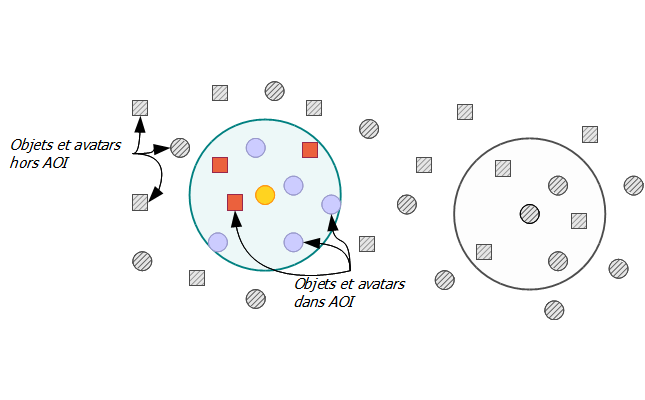
\includegraphics[width=16cm,height=9cm]{../Images/AOI.png}\\
        \caption{Principe de l'\textit{Area Of Interest}}
        \label{AOI}
        \end{figure}
	\vspace{1cm}
\newpage
	\subsection{Découpage de la carte}
	Pour plusieurs raisons, dont la tenue en charge, le monde a été découpé en plusieurs zones. Différentes techniques pour le découpage ont été étudié, l'une des plus courantes est d'utiliser le découpage grâce au découpage de Voronoi,c'est de cette technique que la triangulation de Delaunay s'inspire. Les découpages suivants ces principes sont répandus car un découpage aléatoire ne prendrait pas en compte la densité des objets dans le monde qui peut être très variable entre les régions. Le principe est de découper en zone en fonction de la distance entre les différents objets que se trouve dans l'environnement. Dans une région, on aura un objet qui sera entouré de ces voisins, la limite entre la région de deux voisins se trouve au milieu d'une droite séparant les deux voisins. EXPLIQUER VORONOI et DELAUNAY.\\
	\vspace{1cm}
        \begin{figure}[!h]
        \centering
        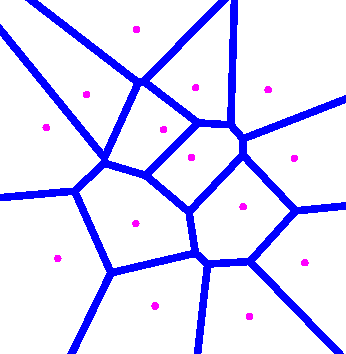
\includegraphics[width=5cm,height=5cm]{../Images/voronoi.png}\\
        \caption{Principe du découpage de Voronoi}
        \label{Voronoi}
        \end{figure}
        \vspace{1cm}
\newpage


	\subsection{revoir fiches lecture} 

	Doppelgängers ????
